\thispagestyle{empty}%
\pdfbookmark{Colophon}{colophon}%
\makeatletter\everypage@\makeatother%
{%
	\small%
	\begin{flushleft}
	Members of the graduation committee:\todo{Verify committee}\\
	\bigskip
	\begin{tabular}{@{}r@{~~}ll}
	Prof.~dr.~ir.\@		& M.\,J.\,G.~Bekooij	& University of Twente (promotor) \\
	Prof.~dr.~ir.\@		& G.\,J.\,M.~Smit		& University of Twente (promotor) \\
	Prof.~dr.\@			& J.\,C.~van~de~Pol		& University of Twente \\
	Dr.~ir.\@			& J.\,F.~Broenink		& University of Twente \\
	Prof.~dr.\@			& H.~Corporaal			& Eindhoven University of Technology \\
	Prof.~dr.~ir.\@		& K.\,L.\,M.~Bertels	& Delft University of Technology \\
	Prof.~dr.~ir.\@		& D.~Stroobandt			& Ghent University \\
	Prof.~dr.\@			& P.\,M.\,G.~Apers		& University of Twente (chairman and secretary) \\
%	\ldots				& \ldots				& \ldots \\
	\end{tabular}

	\vfill
	\todo{Verify print shop, ISBN, ISSN, DOI, and CTIT nr.}

	{%
		\newlength{\logowd}%
		\setlength{\logowd}{27mm}% mind the minimum height of the FSC logo, which is 12mm
		\newlength{\descrwd}%
		\setlength{\descrwd}{\dimexpr\linewidth-\logowd-2\tabcolsep\relax}%
		\begin{tabular}{@{}>{\Centering\arraybackslash\figureversion{text,prop}}m{\logowd}%
						>{\justifying\arraybackslash\noindent\figureversion{text,prop}}m{\descrwd}@{}}
			& %
			\begin{minipage}{\descrwd}%
				\href{http://www.utwente.nl/}{
\includegraphics[width=0.75\linewidth]{figures/ut_logo}} \\[1em]
				Faculty of \acl*{EWI},
				\href{http://caes.ewi.utwente.nl/}{\acf*{CAES}} group
			\end{minipage} \\
			& \\
			\raisebox{-.5ex}{\href{http://www.utwente.nl/ctit}{
\includegraphics[width=\logowd]{figures/ctit_logo}}} & %
			\begin{minipage}[c]{\descrwd}%
				\acs*{CTIT} Ph.D.\ Thesis Series No.\ \thesisCTITnr \\
				\acl*{CTIT} \\
				PO Box 217, 7500 AE {} Enschede, The Netherlands
			\end{minipage} \\
			&\\
%			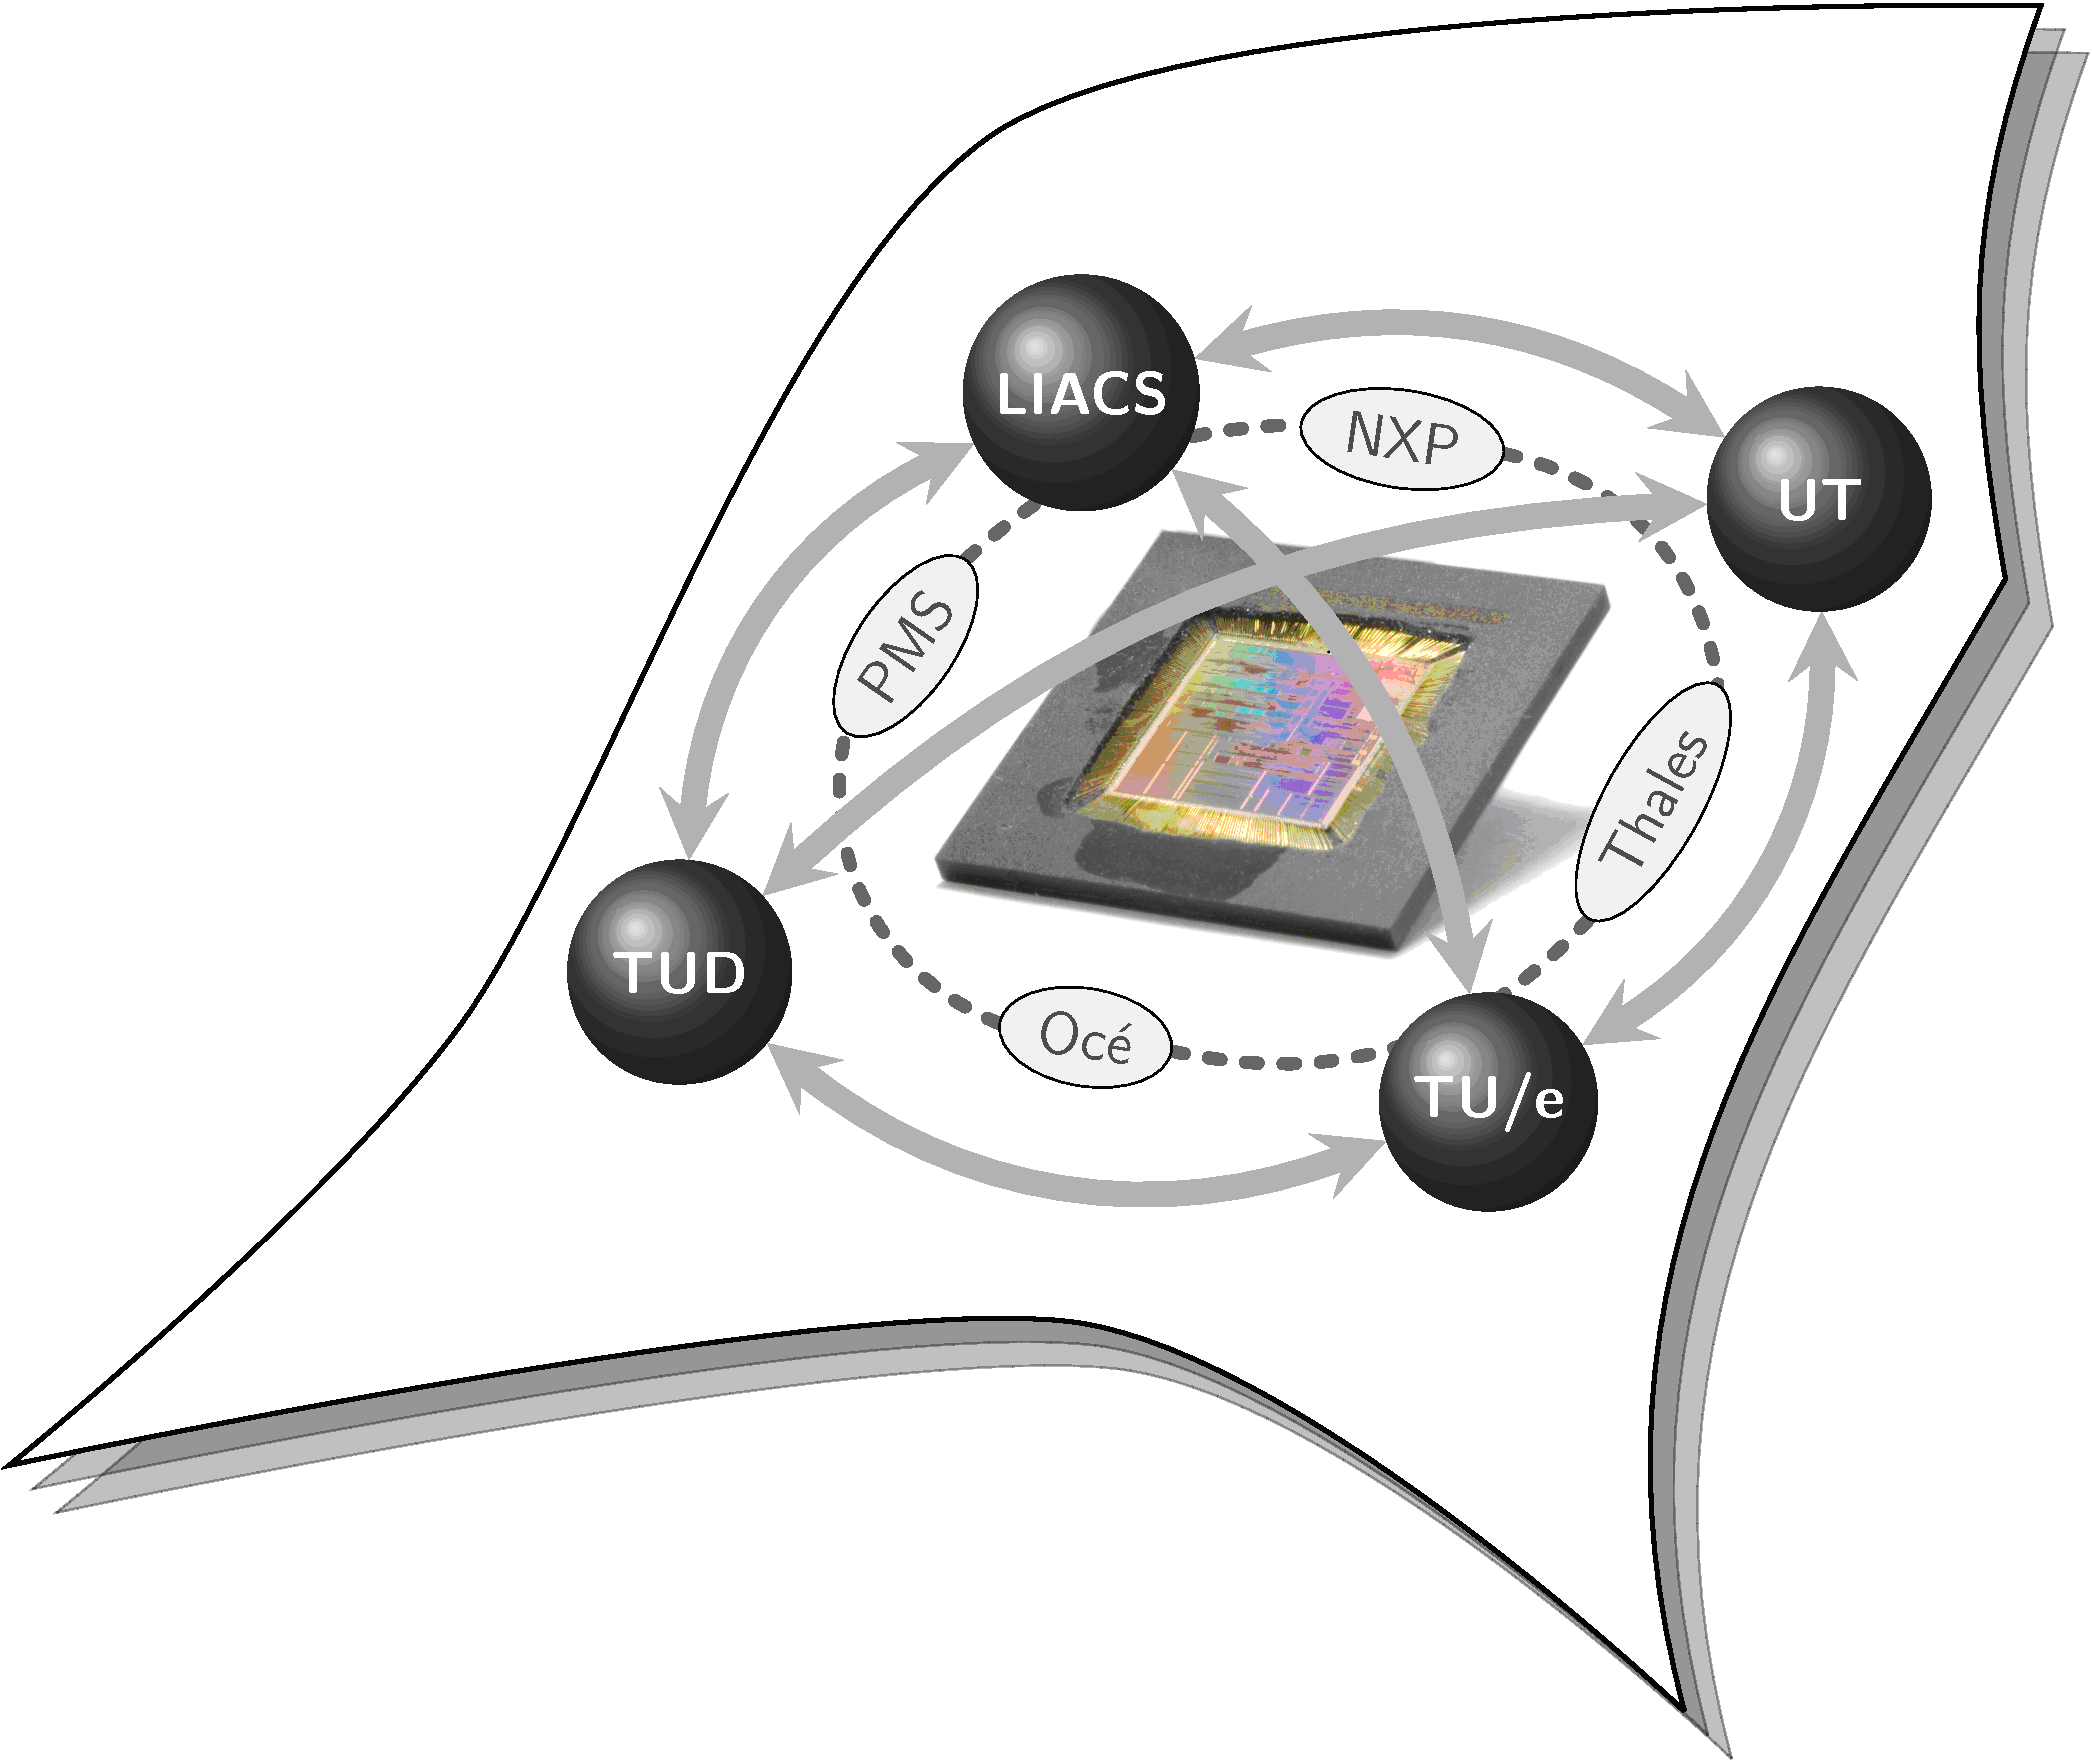
\includegraphics[width=\logowd]{figures/nest_logo}
			\href{http://www.stw.nl/}{
\includegraphics[width=\logowd]{figures/stw_logo}} & %
			\begin{minipage}[c]{\descrwd}%
				This research has been conducted within the \href{http://www.nest-consortium.nl/}{\acf*{NEST}} project (project number 10346).
				This research is supported by the Dutch Technology Foundation \acs*{STW}, which is part of the Netherlands Organisation for Scientific Research (\acs*{NWO}) and partly funded by the Ministry of Economic Affairs.
			\end{minipage} \\
			&\\
			&\\
			\begin{minipage}[c]{\logowd}\centering%
			\begin{tikzpicture}[
				logo/.style={circle,inner sep=0,outer sep=-.025\logowd},
			]
				\node[logo,anchor=270] at (0,0) {
\includegraphics[width=.34\logowd]{figures/cc}};
				\node[logo,anchor=30]  at (0,0) {
\includegraphics[width=.34\logowd]{figures/by}};
				\node[logo,anchor=150] at (0,0) {
\includegraphics[width=.34\logowd]{figures/nc}};% or use nc-eu for euro symbol
			\end{tikzpicture}%
			\end{minipage}%
			& %
			\begin{minipage}[c]{\descrwd}%
				Copyright \copyright\ \thesisyear\ \theauthor, Enschede, The Netherlands.
				This work is licensed under the Creative Commons Attribution-NonCommercial~4.0 International License.
				To view a copy of this license, visit \url{http://creativecommons.org/licenses/by-nc/4.0/deed.en_US}.
			\end{minipage}
			\\
			&\\
			% enable following two lines to show the required minimum height of the FSC logo
%			\tikz[overlay,remember picture]{
%				\draw[red,thick,|<->|] (0,.5\pgflinewidth) to node[sloped,anchor=south,font=\footnotesize] {$\ge$\SI{12}{\milli\meter}} ($(0,12mm)+(0,-.5\pgflinewidth)$);}%
			\mbox{\ifpress\else\expandafter\phantom\fi%
			{\href{http://www.fsc.nl/}{
\includegraphics[height=12.2mm]{figures/FSC_Gildeprint}}}}%
			& %
			\begin{minipage}{\descrwd}%
				This thesis was typeset using \LaTeX, \TikZ, and Vim.
				This thesis was printed by \href{http://www.gildeprint.nl/}{Gildeprint Drukkerijen, The Netherlands}.
			\end{minipage}\\
			&\\
			& \begin{minipage}{\descrwd}%
				\begin{tabular}{@{}l>{\figureversion{text,prop}}l}
				\noac{ISBN} & \thesisISBN \\
				\noac{ISSN} & \href{http://opc4.kb.nl/DB=1/SET=2/TTL=1/CMD?ACT=SRCHA&IKT=1007&SRT=YOP&TRM=\thesisISSN}{\thesisISSN}; %
					\acs*{CTIT} Ph.D.\ Thesis Series No.\ \thesisCTITnr \\
				\noac{DOI}  & \href{http://dx.doi.org/\thesisDOI}{\thesisDOI} \\
				\end{tabular}%
			\end{minipage}\\
		\end{tabular}%
	}%
	\end{flushleft}\vspace{-1.5\baselineskip}\mbox{}%
}%
\clearpage%
